
\part*{Formelsammlung:}


\section*{Analyse der Bilanz}

Kapitalstruktur:
\begin{verse}
\begin{tabular}{|c|c|c|}
\hline 
Name & Formel  & Soll-Wert\tabularnewline
\hline 
\hline 
Fremdfinanzierungsgrad(Verschuldung) & $\frac{Fremdkapital\times100\%}{Gesamtkapital}$ & max 70\%\tabularnewline
\hline 
Eigenfinanzierungsgrad & $\frac{Eigenkapital\times100\%}{Gesamtkapital}$ & min 30\%\tabularnewline
\hline 
Finanzierungsverhältnis & $\frac{Fremdkapital\times100\%}{Eigenkapital}$ & ca. 200-250\%\tabularnewline
\hline 
Selbstfinanzierungsgrad 1 & $\frac{Zuwachskapital\times100\%}{Eigenkapital}$ & prop. zu Alter der Firma\tabularnewline
\hline 
Selbstfinanzierungsgrad 2  & $\frac{Gewinnreserven\times100\%}{Eigenkapital}$ & prop. zu Alter der Firma\tabularnewline
\hline 
\end{tabular}$\frac{}{}$
\end{verse}
Vermögensstruktur:
\begin{verse}
\begin{tabular}{|c|c|c|}
\hline 
Name & Formel  & Soll-Wert\tabularnewline
\hline 
\hline 
Umlaufintensität & $\frac{Umlaufverm\ddot{o}gen\times100\%}{Gesamtverm\ddot{o}gen}$ & branchenabhängig\tabularnewline
\hline 
Anlageintensität (Alter der Anlagen bek.) & $\frac{Anlageverm\ddot{o}gen\times100\%}{Gesamtverm\ddot{o}gen}$ & branchenabhängig\tabularnewline
\hline 
Investitionsverhältnis & $\frac{Umlaufverm\ddot{o}gen\times100\%}{Anlageverm\ddot{o}gen}$ & branchenabhängig\tabularnewline
\hline 
Anlageabnutzungsgrad & $\frac{Kummulierte\, Abschreibungen}{Anschaffungswert}$ & je höher, je ältere Firma\tabularnewline
\hline 
\end{tabular}
\end{verse}
Liquidität:
\begin{verse}
\begin{tabular}{|>{\centering}p{5cm}|c|c|}
\hline 
Name & Formel  & Soll-Wert\tabularnewline
\hline 
\hline 
Liquiditätsgrad 1, Cash Ratio & $\frac{Liquide-Mittel\times100\%}{Kurzfristiges-Fremdkapital}$ & ca. 30-50\%\tabularnewline
\hline 
Liquiditätsgrad 2, Quick Ratio & $\frac{(Fl.\, Mittel+Wertschriften+(Geld)Forderungen+akt.\, Rech.abgr.)\times100\%}{Kurzfristiges-Fremdkapital}$ & $>$100\%\tabularnewline
\hline 
Liquiditätsgrad 3, Current Ratio (LQ2+Vorräte) & $\frac{Umlaufverm\ddot{o}gen\times100\%}{Kurzfristiges-Fremdkapital}$ & 150-200\%\tabularnewline
\hline 
\end{tabular}
\end{verse}
Anlagedeckung (goldene Bilanzregel):
\begin{verse}
\begin{tabular}{|c|c|c|}
\hline 
Name & Formel  & Soll-Wert\tabularnewline
\hline 
\hline 
Anlage Deckungsgrad 1  & $\frac{Eigenkapital\times100\%}{Anlageverm\ddot{o}gen}$ & 75-100\%\tabularnewline
\hline 
Anlage Deckungsgrad 2  & $\frac{(Eigenkap.+langfr.-Fremdkapital)\times100\%}{Anlageverm\ddot{o}gen}$ & $>$100\%\tabularnewline
\hline 
\end{tabular}
\end{verse}

\section*{Erfolgsbezogene Analyse (Rentabilität)}

Rentabilität:
\begin{verse}
\begin{tabular}{|c|c|c|}
\hline 
Name & Formel  & Soll-Wert\tabularnewline
\hline 
\hline 
Rentabilität (allg) & $\frac{Erfolg(pro.Jahr)\times100\%}{\oslash Kapitaleinsatz}$ & \tabularnewline
\hline 
Gesamtkapitalrentabilität (brutto) & $\frac{EBIT(Gewinn\, vor\, Steuer)\times100\%}{\oslash Gesamtkapital(total\, Passiven\oslash)}$ & $>6\%$\tabularnewline
\hline 
Eigenkapitalrentabilität (netto) & $\frac{Unternehmungsgewinn\times100\%}{\oslash Eigenkapital(Akt+Res+Gew)}$ & $>8\%$\tabularnewline
\hline 
Betriebskapitalrentabilität & $\frac{Betriebsgewinn\times100\%}{\oslash Betriebskapital}$ & \tabularnewline
\hline 
\end{tabular}
\end{verse}

\section*{Aktivitätsbezogene Analyse}
\begin{verse}
\begin{tabular}{|c|c|c|}
\hline 
Name & Formel  & Soll-Wert\tabularnewline
\hline 
\hline 
Debitorenumschlag & $\frac{Kreditverkaufsumsatz}{\oslash Debitorenbestand}=\frac{Nettoumsatz}{\oslash Forderungen\, L+L}$ & max\tabularnewline
\hline 
$\oslash$Debitorenfrist & $\frac{360d}{Debitorenumschlag}$ & min\tabularnewline
\hline 
Kreditorenumschlag & $\frac{Krediteinkauf}{\oslash Kreditorenbestand}=\frac{Krediteinkauf}{\oslash Verbindlichkeiten\, L+L}$ & min\tabularnewline
\hline 
$\oslash$Kreditorenfrist & $\frac{360d}{Kreditorenumschlag}$ & max\tabularnewline
\hline 
Lagerumschlag & $\frac{Warenaufwand}{\oslash Warenbestand\,(Vorr\ddot{a}te)}$ & max\tabularnewline
\hline 
$\oslash$Lagerdauer & $\frac{360d}{Lagerumschlag}$ & min\tabularnewline
\hline 
\end{tabular}
\end{verse}

\section*{Analyse von börsenkotierten Aktien und Unternehmen}
\begin{verse}
\begin{tabular}{|c|c|c|}
\hline 
Name & Formel  & Soll-Wert\tabularnewline
\hline 
\hline 
Börsenkapitalisierung & $Anzahl\, ausstehender\, Aktien\times Kurs$ & \tabularnewline
\hline 
Gewinn je Aktie & $\frac{Jahresgewinn\,(Konzerngewinn-Minderheiten)}{\oslash Anzahl\, ausstehender\, Aktien}$ & \tabularnewline
\hline 
Kurs-Gewinn-Verhältniss (P/E Ratio) & $\frac{Kurs}{Gewinn\, je\, Aktien\,(EPS)}$ & \tabularnewline
\hline 
Gewinnrendite & $\frac{Gewinn\, je\, Aktie\,(EPS)\times100\%}{Kurs}$ & \tabularnewline
\hline 
\end{tabular}
\end{verse}

\section*{Analyse Mittelflussrechnung}

\begin{tabular}{|c|c|c|}
\hline 
Name & Formel  & Soll-Wert\tabularnewline
\hline 
\hline 
Re-Investment-Faktor (Investitionsgrad) & $\frac{Nettoinvestitionen\times100\%}{Cash\, Flow}$ & \tabularnewline
\hline 
Cash Flow Marge & $\frac{Cash\, Flow\times100\%}{Umsatz}$ & \tabularnewline
\hline 
\end{tabular}


\section*{EBITA etc}

\begin{tabular}{ll}
$Verkaufsumsatz$ & $Krediteinkauf=Warenaufwand\:\pm Lagerver\ddot{a}nderung$\tabularnewline
$-Warenaufwand$ & $Gewinn=Erl\ddot{o}s-Kosten$\tabularnewline
$=Bruttogewinn$ & $Rohgewinn=Erl\ddot{o}s-Liquidit\ddot{a}tswirksame\, Kosten\,(Kapitalkosten+Abschreibungen)$\tabularnewline
$-Versch.\, Gemerinaufwand$ & \tabularnewline
$=EBITDA$ & \tabularnewline
$-Abschreibungen$ & \tabularnewline
$=EBIT$ & \tabularnewline
$-Fremdkapitalzins$ & \tabularnewline
$=EBT$ & \tabularnewline
$-Steuern$ & \tabularnewline
$=EAT$ & \tabularnewline
\end{tabular}


\section*{Leverage-Effekt}

Ein niedriger Anteil an Eigenkapital bzw. ein hoher Anteil an Fremdkapital
kann sich hingegen positiv auf die Rentabilität auswirken, solange
die Gesamtkapitalrentabilität ($\frac{EBIT}{Gesamtkapital}$) höher
ist, als der durchschnittliche für das Fremdkapital zu bezahlende
Zinssatz. Dieser Effekt wird ``Leverage-Effekt'' oder ``Hebelwirkung
des Fremdkapitals'' genannt.

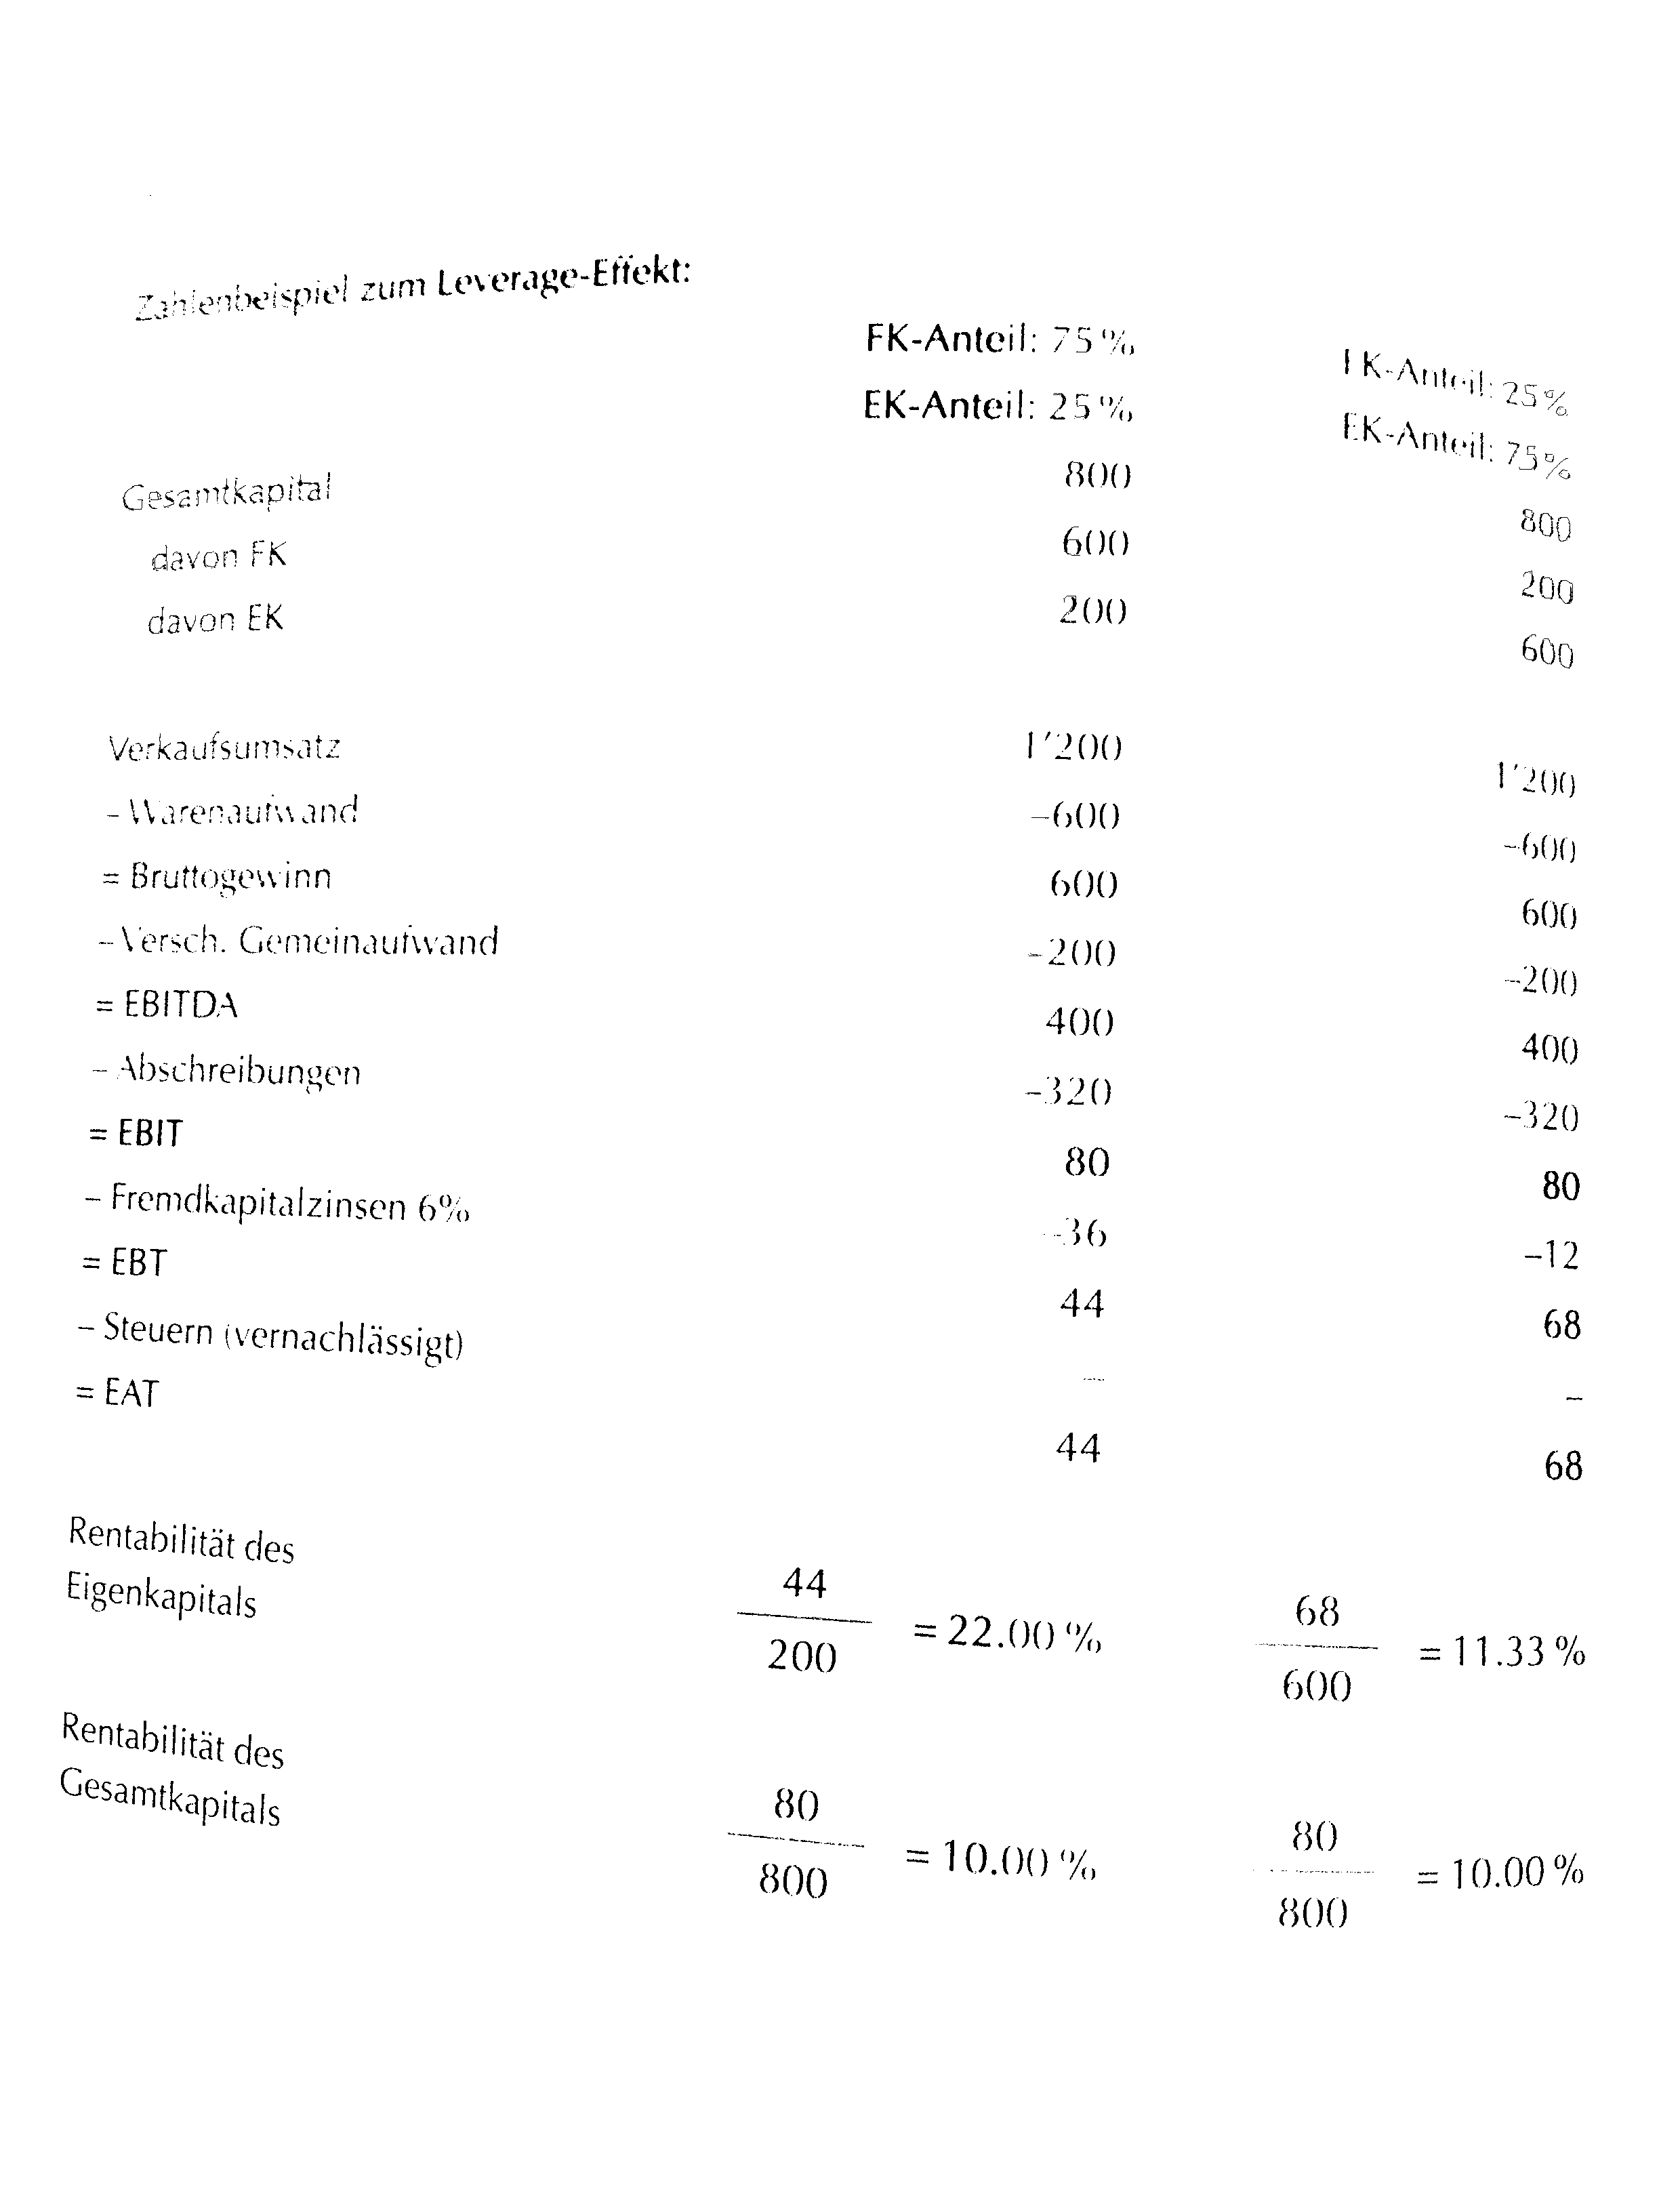
\includegraphics[width=17cm]{AnalyseJahresabschluss/Leverage}
